\documentclass[10pt]{article}
\usepackage{geometry}
\usepackage{graphicx}
\usepackage{natbib}
\usepackage{amsmath}
\usepackage{amssymb}
\usepackage{amsthm}
\usepackage{paralist}
\usepackage{epstopdf}
\usepackage{tabularx}
\usepackage{longtable}
\usepackage{multirow}
\usepackage{multicol}
\usepackage[hidelinks]{hyperref}
\usepackage{fancyvrb}
\usepackage{algorithm}
\usepackage{algorithmic}
\usepackage{float}
\usepackage[svgname]{xcolor}
\usepackage{enumerate}
\usepackage{array}
\usepackage{url}
\usepackage{fancyhdr}
\usepackage{comment}
\usepackage{environ}
\usepackage{times}
\usepackage{textcomp}
\usepackage{caption}
\usepackage{bbm}
\usepackage{enumitem}
\usepackage{ctex} 
\usepackage{subfigure}
% 以下是新增的自定义格式更改
% \usepackage[]{caption2} %新增调用的宏包
\renewcommand{\figurename}{Fig.} %重定义编号前缀词
% \renewcommand{\captionlabeldelim}{.~} %重定义分隔符
% \roman是罗马数字编号,\alph是默认的字母编号,\arabic是阿拉伯数字编号,可按需替换下一行的相应位置
\renewcommand{\thesubfigure}{(\roman{subfigure})} %此外,还可设置图编号显示格式,加括号或者不加括号
\makeatletter \renewcommand{\@thesubfigure}{\thesubfigure \space} %子图编号与名称的间隔设置
\renewcommand{\p@subfigure}{} \makeatother

\urlstyle{rm}

\setlength\parindent{0pt} % Removes all indentation from paragraphs
\theoremstyle{definition}
\newtheorem{definition}{Definition}[]
\newtheorem{conjecture}{Conjecture}[]
\newtheorem{example}{Example}[]
\newtheorem{theorem}{Theorem}[]
\newtheorem{lemma}{Lemma}
\newtheorem{proposition}{Proposition}
\newtheorem{corollary}{Corollary}

\floatname{algorithm}{Procedure}
\renewcommand{\algorithmicrequire}{\textbf{Input:}}
\renewcommand{\algorithmicensure}{\textbf{Output:}}
\newcommand{\abs}[1]{\lvert#1\rvert}
\newcommand{\norm}[1]{\lVert#1\rVert}
\newcommand{\RR}{\mathbb{R}}
\newcommand{\CC}{\mathbb{C}}
\newcommand{\Nat}{\mathbb{N}}
\newcommand{\br}[1]{\{#1\}}
\DeclareMathOperator*{\argmin}{arg\,min}
\DeclareMathOperator*{\argmax}{arg\,max}
\renewcommand{\qedsymbol}{$\blacksquare$}

\definecolor{dkgreen}{rgb}{0,0.6,0}
\definecolor{gray}{rgb}{0.5,0.5,0.5}
\definecolor{mauve}{rgb}{0.58,0,0.82}

\newcommand{\Var}{\mathrm{Var}}
\newcommand{\Cov}{\mathrm{Cov}}

\newcommand{\vc}[1]{\boldsymbol{#1}}
\newcommand{\xv}{\vc{x}}
\newcommand{\Sigmav}{\vc{\Sigma}}
\newcommand{\alphav}{\vc{\alpha}}
\newcommand{\muv}{\vc{\mu}}

\newcommand{\red}[1]{\textcolor{red}{#1}}

\def\x{\mathbf x}
\def\y{\mathbf y}
\def\w{\mathbf w}
\def\v{\mathbf v}
\def\E{\mathbb E}
\def\V{\mathbb V}
\def\ind{\mathbbm 1}

% TO SHOW SOLUTIONS, include following (else comment out):
\newenvironment{soln}{
    \leavevmode\color{blue}\ignorespaces
}{}


\hypersetup{
%    colorlinks,
    linkcolor={red!50!black},
    citecolor={blue!50!black},
    urlcolor={blue!80!black}
}

\geometry{
  top=1in,            % <-- you want to adjust this
  inner=1in,
  outer=1in,
  bottom=1in,
  headheight=3em,       % <-- and this
  headsep=2em,          % <-- and this
  footskip=3em,
}


\pagestyle{fancyplain}
\lhead{\fancyplain{}{Homework 4}}
\rhead{\fancyplain{}{CS 760 Machine Learning}}
\cfoot{\thepage}

\title{\textsc{Homework 4}} % Title

%%% NOTE:  Replace 'NAME HERE' etc., and delete any "\red{}" wrappers (so it won't show up as red)

\author{
Yuhan Wang \\
ywang2558 \\
} 

\date{}

\begin{document}

\maketitle


\textbf{Instructions:} Use this latex file as a template to develop your homework. Submit your homework on time as a single pdf file to Canvas. Late submissions may not be accepted. Please wrap your code and upload it to a public GitHub repo, then attach the link below the instructions so that we can access it. You can choose any programming language (i.e. python, R, or MATLAB). Please check Piazza for updates about the homework.\\

Github link: \url{https://github.com/hanhuangv587/CS760hw4}\\

\section{Best Prediction}
\subsection{Under 0-1 Loss (10 pts)}
Suppose the world generates a single observation $x \sim \mbox{multinomial}(\theta)$, where the parameter vector $\theta=(\theta_1, \ldots, \theta_k)$ with $\theta_i\ge 0$ and $\sum_{i=1}^k \theta_i=1$.  Note $x \in \{1, \ldots, k\}$.
You know $\theta$ and want to predict $x$.
Call your prediction $\hat x$.  What is your expected 0-1 loss:
$$\E[\ind_{\hat x \neq x}]$$
using the following two prediction strategies respectively?  Prove your answer.
\begin{enumerate}
    \item Strategy 1: $\hat x \in \argmax_x \theta_x$, the outcome with the highest probability.

          \begin{soln}
              $$\E[\ind_{\hat x \neq x}] = 1 - P(x = \hat x) = 1 - \max_x \theta_x$$
          \end{soln}

    \item Strategy 2: You mimic the world by generating a prediction $\hat x \sim \mbox{multinomial}(\theta)$.  (Hint: your randomness and the world's randomness are independent)

          \begin{soln}
              $$\E[\ind_{\hat x \neq x}] = 1 - \sum_{i=1}^{k} P(x = i, \hat x = i) = 1 - \sum_{i=1}^{k} \theta_i^2 $$
          \end{soln}

\end{enumerate}

\subsection{Under Different Misclassification Losses (6 pts)}
Like in the previous question, the world generates a single observation $x \sim \mbox{multinomial}(\theta)$. Let $c_{ij} \ge 0$ denote the loss you incur, if $x=i$ but you predict $\hat x=j$, for $i,j \in \{1, \ldots, k\}$.
$c_{ii}=0$ for all $i$. This is a way to generalize different costs of false positives vs false negatives from binary classification to multi-class classification. You want to minimize your expected loss:
$$\E[c_{x \hat x}].$$
Derive your optimal prediction $\hat x$.

\begin{soln}
    \begin{align*}
        \E[c_{x \hat x}] & = \sum_{i=1}^{k} \sum_{j=1}^{k} c_{ij} P(x = i, \hat x = j)           \\
                         & = \sum_{i=1}^{k} \sum_{j=1}^{k} \theta_i c_{ij} P(\hat x = j | x = i) \\
                         & = \sum_{i=1}^{k} \sum_{j=1}^{k} \theta_i c_{ij} P(\hat x = j)         \\
    \end{align*}
    Let $p_1, \dots , p_k$ be the probabilities of $P(\hat x)$. Then the optimization problem is:
    \begin{align*}
        \min_{\hat x} \sum_{i=1}^{k}   & \sum_{j=1}^{k} \theta_i c_{ij} p_j \\
        \text{s.t.} \sum_{j=1}^{k} p_j & = 1,                               \\
        p_j \ge 0, j                   & = 1, \dots , k                     \\
    \end{align*}
    This is a linear programming problem. We can solve it by the simplex method. The optimal solution is:
    \begin{align*}
        p_j = 1, j = \argmin_{i} \sum_{i=1}^{k} \theta_i c_{ij}, \\
        p_j = 0, j \neq \argmin_{i} \sum_{i=1}^{k} \theta_i c_{ij}.
    \end{align*}
\end{soln}


\section{Language Identification with Naive Bayes (8 pts each)}
Implement a character-based Naive Bayes classifier that classifies a document as English, Spanish, or Japanese - all written with 26 lower-case characters and space.

The dataset is languageID.tgz, unpack it. This dataset consists of 60 documents in English, Spanish, and Japanese. The correct class label is the first character of the filename: $y \in \{e, j, s\}$. (Note: here each file is a document in the corresponding language, and it is regarded as one data.)

We will be using a character-based multinomial Naïve Bayes model. You need to view each document as a bag of characters, including space. We have made sure that there are only 27 different types of printable characters (a to z, and space) -- there may be additional control characters such as new-line, please ignore those. Your vocabulary will be these 27 character types. (Note: not word types!)

In the following questions, you may use the additive smoothing technique to smooth categorical data, in case the estimated probability is zero. Given $N$ data samples $\{\vc{x}^{(i)}, y^{(i)}\}_{i = 1}^{N}$, where $\vc{x}^{(i)} = [x_1^{(i)}, \dots, x_j^{(i)}, \dots, x_{M_i}^{(i)}]$ is a bag of characters, $M_i$ is the total number of characters in $\vc{x}^{(i)}$, $x_{j}^{(i)} \in S, y^{(i)} \in L$ and we have $|S| = K_S, |L| = K_L$. Here $S$ is the set of all character types, and $L$ is the set of all classes of data labels. Then by the additive smoothing with parameter $\alpha$, we can estimate the conditional probability as
$$
    P_{\alpha}(a_s \mid y = c_k) = \frac{(\sum_{i = 1}^{N}\sum_{j = 1}^{M_i}\ind [x_{j}^{(i)} = a_s, y^{(i)} = c_k]) + \alpha}{(\sum_{b_s \in S}\sum_{i = 1}^{N}\sum_{j = 1}^{M_i}\ind [x_{j}^{(i)} = b_s, y^{(i)} = c_k]) + K_S \alpha},
$$
where $a_s \in S, c_k \in L$. Similarly, we can estimate the prior probability
$$
    P_{\alpha}(Y = c_k) = \frac{(\sum_{i = 1}^{N}\ind [y^{(i)} = c_k]) + \alpha}{N + K_L \alpha},
$$
where $c_k \in L$ and $N$ is the number of training samples.
\begin{enumerate}
    \item
          Use files 0.txt to 9.txt in each language as the training data.
          Estimate the prior probabilities
          $\hat p(y=e)$,
          $\hat p(y=j)$,
          $\hat p(y=s)$
          using additive smoothing with parameter $\frac{1}{2}$.
          Give the formula for additive smoothing with parameter $\frac{1}{2}$ in this case.
          Print the prior probabilities.

          \begin{soln}
              Since the numbers of files in each language are the same in the training data, $\hat p(y=e) = \hat p(y=j) = \hat p(y=s) = \frac{1}{3}$
          \end{soln}

    \item
          Using the same training data, estimate the class conditional probability (multinomial parameter) for English
          $$\theta_{i,e} := \hat p(c_i \mid y=e)$$
          where $c_i$ is the $i$-th character. That is, $c_1 = a, \ldots, c_{26} = z, c_{27} = space$.
          Again, use additive smoothing with parameter $\frac{1}{2}$.
          Give the formula for additive smoothing with parameter $\frac{1}{2}$ in this case.
          Print $\theta_e$ which is a vector with 27 elements.

          \begin{soln}
              $\theta_e$ = [0.0616 0.012  0.0217 0.0219 0.1075 0.0202 0.0145 0.0478 0.0524 0.0006
              0.0043 0.031  0.0228 0.056  0.0663 0.0155 0.0008 0.0488 0.0622 0.0868
              0.025  0.009  0.0161 0.0011 0.0134 0.0005 0.1802]

          \end{soln}

    \item
          Print $\theta_j, \theta_s$, the class conditional probabilities for Japanese and Spanish.

          \begin{soln}
              $\theta_j$ = [1.3168e-01 9.1100e-03 5.7000e-03 1.5940e-02 5.9950e-02 3.2400e-03
              1.6140e-02 3.1150e-02 1.0035e-01 2.2900e-03 5.7020e-02 9.2000e-04
              4.1190e-02 5.6000e-02 8.9850e-02 9.9000e-04 3.0000e-05 4.3440e-02
              4.1530e-02 5.9410e-02 6.9170e-02 1.7000e-04 2.0510e-02 3.0000e-05
              1.4090e-02 7.4000e-03 1.2274e-01] \\
              $\theta_s$ = [0.1035 0.0103 0.0365 0.0422 0.1149 0.0072 0.0067 0.005  0.0503 0.0064
              0.0002 0.0511 0.0244 0.0557 0.0703 0.0251 0.0081 0.0578 0.0676 0.035
              0.0363 0.0059 0.0004 0.0023 0.0059 0.004  0.1671]
          \end{soln}

    \item
          Treat e10.txt as a test document $x$.
          Represent $x$ as a bag-of-words count vector (Hint: the vocabulary has size 27).
          Print the bag-of-words vector $x$.

          \begin{soln}
              x = [126  16  31  37 166  32  21  57  98   0   7  57  43 100  90  29   0  84
              105 118  46  15  24   3  23   1 302]
          \end{soln}

    \item
          For the $x$ of e10.txt, compute $\hat p(x \mid y)$ for $y=e, j, s$ under the multinomial model assumption, respectively.
          Use the formula
          $$\hat p(x \mid y) = \prod_{i=1}^d (\theta_{i, y})^{x_i}$$
          where $x=(x_1, \ldots, x_d)$.
          Show the three values: $\hat p(x \mid y=e), \hat p(x \mid y=j), \hat p(x \mid y=s)$.

          Hint: you may notice that we omitted the multinomial coefficient.  This is ok for classification because it is a constant w.r.t. $y$. Also, Store all probabilities here and below in $\log()$ internally to avoid underflow. This also means you need to do arithmetic in log space.

          \begin{soln}
              \begin{align*}
                  \hat p(x \mid y=e) = e^{-4598.296} \\
                  \hat p(x \mid y=j) = e^{-5109.846} \\
                  \hat p(x \mid y=s) = e^{-4838.794}
              \end{align*}
          \end{soln}

    \item
          For the $x$ of e10.txt, use the Bayes rule and your estimated prior and likelihood, compute the posterior $\hat p(y \mid x)$.
          Show the three values: $\hat p(y=e \mid x), \hat p(y=j \mid x), \hat p(y=s \mid x)$.
          Show the predicted class label of $x$.

          \begin{soln}
              The predicted class label of $x$ is English.
          \end{soln}

    \item
          Evaluate the performance of your classifier on the test set (files 10.txt to 19.txt in three languages).
          Present the performance using a confusion matrix. A confusion matrix summarizes the types of errors your classifier makes, as shown in the table below.   The columns are the true language a document is in, and the rows are the classified outcome of that document.  The cells are the number of test documents in that situation.  For example, the cell with row = English and column = Spanish contains the number of test documents that are really Spanish but misclassified as English by your classifier.

          \begin{center}
              \begin{tabular}{c|ccc}
                           & English & Spanish & Japanese \\
                  \hline
                  English  & 10      &         &          \\
                  Spanish  &         & 10      &          \\
                  Japanese &         &         & 10
              \end{tabular}
          \end{center}

    \item Take a test document.   Arbitrarily shuffle the order of its characters so that the words (and spaces) are scrambled beyond human recognition.  How does this shuffling affect your Naive Bayes classifier's prediction on this document?  Explain the key mathematical step in the Naive Bayes model that justifies your answer.

          \begin{soln}
              The shuffling of the characters in the document will not affect the prediction of the Naive Bayes classifier. The Naive Bayes classifier is based on the conditional independence of the characters in the document. The shuffling of the characters in the document will not affect the conditional independence of the characters in the document.
          \end{soln}

\end{enumerate}

\section{Simple Feed-Forward Network (20pts)}
In this exercise, you will derive, implement back-propagation for a simple neural network and compare your output with some standard library’s output. Consider the following 3-layer neural network.

\[
    \hat{y} = f(x) = g(W_3\sigma(W_2\sigma(W_1x)))
\]

Suppose $x \in \mathbb{R}^d$, $W_1 \in \mathbb{R}^{d_1 \times d}$, $W_2 \in \mathbb{R}^{d_2 \times d_1}$, $W_3 \in \mathbb{R}^{k \times d_2}$ i.e. $f: \mathbb{R}^d \rightarrow \mathbb{R}^k$, Let $\sigma(z) = [\sigma(z_1), ..., \sigma(z_n)]$ for any $z \in \mathbb{R}^n$ where $\sigma(z) = \frac{1}{1 + e^{-z}}$ is the sigmoid (logistic) activation function and $g(z_i) = \frac{exp(z_i)}{\sum_{i=1}^k exp(z_i)}$ is the softmax function. Suppose the true pair is $(x, y)$ where $y \in \{0, 1\}^k$ with exactly one of the entries equal to 1, and you are working with the cross-entropy loss function given below,

\[
    L(x, y) = -\sum_{i=1}^k y \text{log}(\hat{y})
\]

\begin{enumerate}
    \item Derive backpropagation updates for the above neural network. (5 pts) \\
          \begin{soln}
              Let $z_1 = W_1x$, $z_2 = W_2\sigma(z_1)$, $z_3 = W_3\sigma(z_2)$, $\hat{y} = g(z_3)$, $h_1 = \sigma(z_1)$ and $h_2 = \sigma(z_2)$. \\
              \begin{align*}
                  \frac{\partial L}{\partial W_3} & = \frac{\partial L}{\partial \hat{y}} \frac{\partial \hat{y}}{\partial W_3}                                                                                     \\
                                                  & = \frac{\partial L}{\partial \hat{y}} \frac{\partial \hat{y}}{\partial z_3} \frac{\partial z_3}{\partial W_3}                                                   \\
                                                  & = (\hat{y} - y) \sigma(z_2) ^ T                                                                                                                                 \\
                  \frac{\partial L}{\partial W_2} & = \frac{\partial L}{\partial \hat{y}} \frac{\partial \hat{y}}{\partial W_2}                                                                                     \\
                                                  & = \frac{\partial L}{\partial \hat{y}} \frac{\partial \hat{y}}{\partial z_3} \frac{\partial z_3}{\partial \sigma(z_2)} \frac{\partial \sigma(z_2)}{\partial W_2} \\
                                                  & = W_3 ^ T (\hat{y} - y)  \sigma(z_2) ^ T (1 - \sigma(z_2)) \sigma(z_1) ^ T                                                                                      \\
                  \frac{\partial L}{\partial W_1} & = \frac{\partial L}{\partial \hat{y}} \frac{\partial \hat{y}}{\partial W_1}                                                                                     \\
                                                  & = \frac{\partial L}{\partial \hat{y}} \frac{\partial \hat{y}}{\partial z_3} \frac{\partial z_3}{\partial \sigma(z_2)} \frac{\partial \sigma(z_2)}{\partial W_1} \\
                                                  & = W_2 ^ T  W_3 ^ T (\hat{y} - y)  \sigma(z_2) ^ T (1 - \sigma(z_2)) \sigma(z_1) ^ T (1 - \sigma(z_1)) x ^ T                                                     \\
                                                  & = W_2 ^ T  W_3 ^ T (\hat{y} - y)  \sigma(z_2) ^ T (1 - \sigma(z_2)) \sigma(z_1) ^ T (1 - \sigma(z_1)) x ^ T
              \end{align*}
          \end{soln}
    \item Implement it in NumPy or PyTorch using basic linear algebra operations. (e.g. You are not allowed to use auto-grad, built-in optimizer, model, etc. in this step. You can use library functions for data loading, processing, etc.). Evaluate your implementation on MNIST dataset, report test errors and learning curve. (10 pts) \\
          \begin{soln}
              test error = 0.2628 \\
              optimizer = SGD \\
              batch size = 64 \\
              learning rate = 0.004 \\
              epochs = 500 \\
              \begin{figure}[H]
                \centering  %图片全局居中
                \subfigure[epoch vs loss]{
                \label{Fig1.sub.1}
                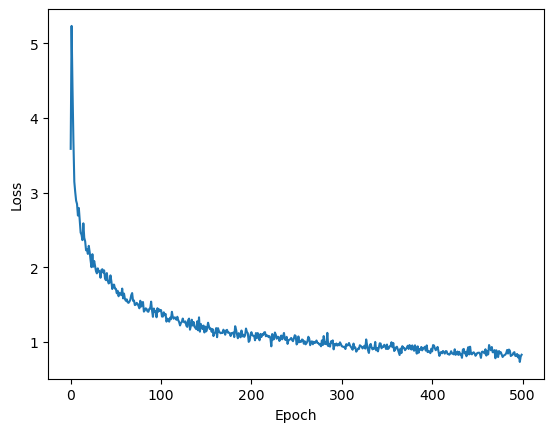
\includegraphics[width=0.45\textwidth]{Fig3.png}}
                \subfigure[epoch vs accuracy]{
                \label{Fig1.sub.2}
                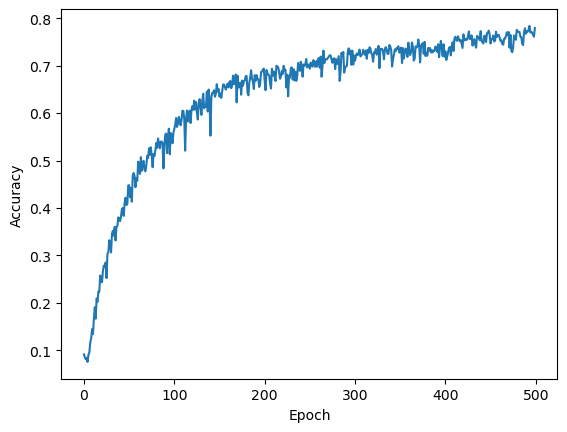
\includegraphics[width=0.45\textwidth]{Fig4.png}}
                \caption{Learning curve for hand implementation, initialize the weights randomly between -1 and 1}
                \label{Fig1.main}
              \end{figure}
          \end{soln}
    \item Implement the same network in PyTorch (or any other framework). You can use all the features of the framework e.g. auto-grad etc. Evaluate it on MNIST dataset, report test errors, and learning curve. (2 pts) \\
          \begin{soln}
              test error = 0.1168 \\
              optimizer = Adam \\
              epochs = 200 \\
              \begin{figure}[H]
                \centering  %图片全局居中
                \subfigure[epoch vs loss]{
                \label{Fig2.sub.1}
                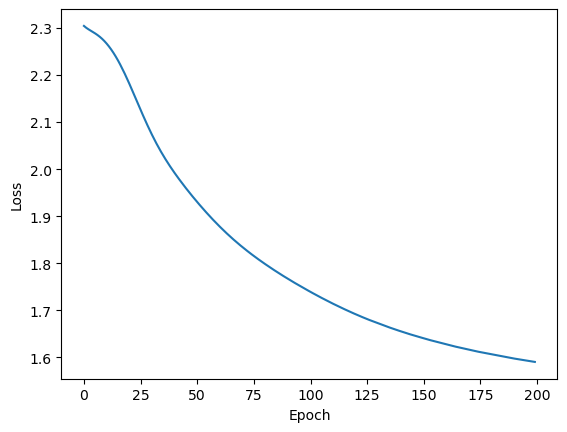
\includegraphics[width=0.45\textwidth]{Fig5.png}}
                \subfigure[epoch vs accuracy]{
                \label{Fig2.sub.2}
                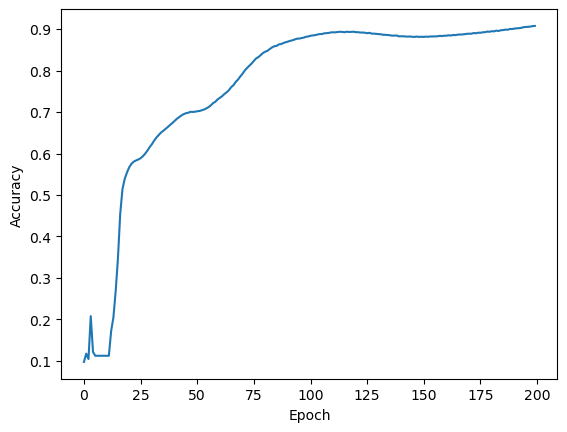
\includegraphics[width=0.45\textwidth]{Fig6.png}}
                \caption{Learning curve for PyTorch implementation}
                \label{Fig2.main}
              \end{figure}
          \end{soln}
    \item Try different weight initialization a) all weights initialized to 0, and b) initialize the weights randomly between -1 and 1. Report test error and learning curves for both. (You can use either of the implementations) (3 pts) \\
          \begin{soln}
            b) is shown in q3.2 with learning rate = 0.004, batch size = 64, epochs = 500 \\
            a) is shown below with learning rate = 0.004, batch size = 64, epochs = 500 \\
            test error = 0.9042 \\
            \begin{figure}[H]
                \centering  %图片全局居中
                \subfigure[epoch vs loss]{
                \label{Fig3.sub.1}
                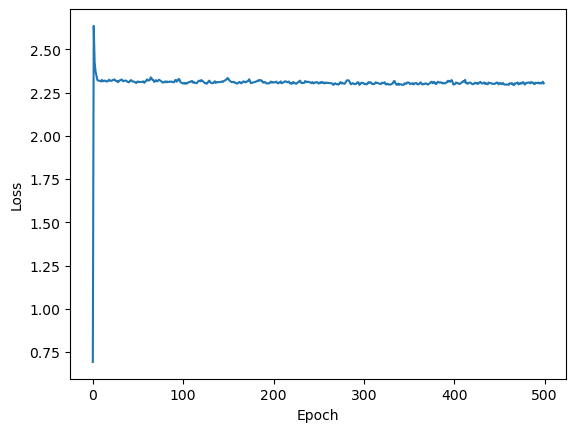
\includegraphics[width=0.45\textwidth]{Fig1.png}}
                \subfigure[epoch vs accuracy]{
                \label{Fig3.sub.2}
                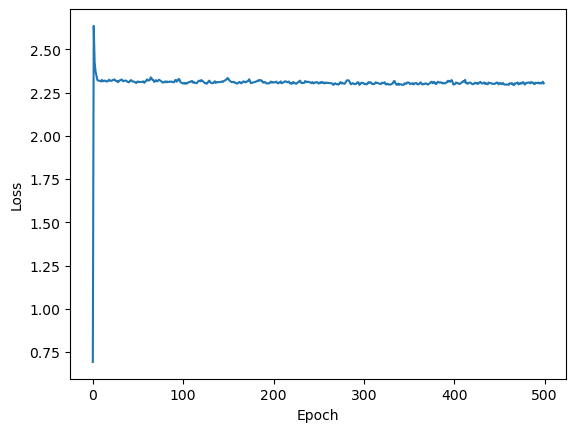
\includegraphics[width=0.45\textwidth]{Fig1.png}}
                \caption{Learning curve for all weights initialized to 0}
                \label{Fig3.main}
              \end{figure}
          \end{soln}
\end{enumerate}

You should play with different hyperparameters like learning rate, batch size, etc. for your own learning. You only need to report results for any particular setting of hyperparameters. You should mention the values of those along with the results. Use $d_1 = 300$, $d_2 = 200$, $d_3 = 100$. For optimization use SGD (Stochastic gradient descent) without momentum, with some batch size say 32, 64, etc. MNIST can be obtained from here (https://pytorch.org/vision/ stable/datasets.html)

\bibliographystyle{apalike}
\end{document}
